\chapter*{Anexo}
\addcontentsline{toc}{chapter}{Anexo}
\markboth{Anexo}{Anexo}
\section*{Problemas interactivos}
\addcontentsline{toc}{section}{Problemas interactivos}
\label{interactivos}

Los problemas interactivos son unos problemas que se resuelven ligeramente diferente a los tradicionales.

En un problema tradicional, uno lee los datos, los procesa y luego obtenemos información de salida.
\begin{center}	
	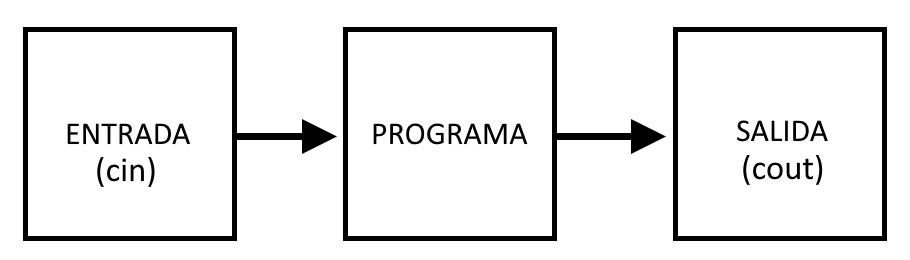
\includegraphics[scale=0.4]{ioproblem}
\end{center}

Pero esto no es como funciona en los problemas interactivos. En estos, puedes imaginar que hay dos programas, uno que es el juez y otro que es el tuyo.

Podemos imaginarlo como dos personas, una eres tú y la otra es el juez.

El juez te pedirá que hagas algo, como encontrar un número secreto. Y tu deberás hacer lo que te pide, pero también podrás pedirle favores al juez, ya sea que haga algo o que te responda una pregunta. Es decir, a diferencia de los problemas estándar, aquí puedes interactuar con el juez.

El flujo de información va en dos sentidos.

\begin{center}	
	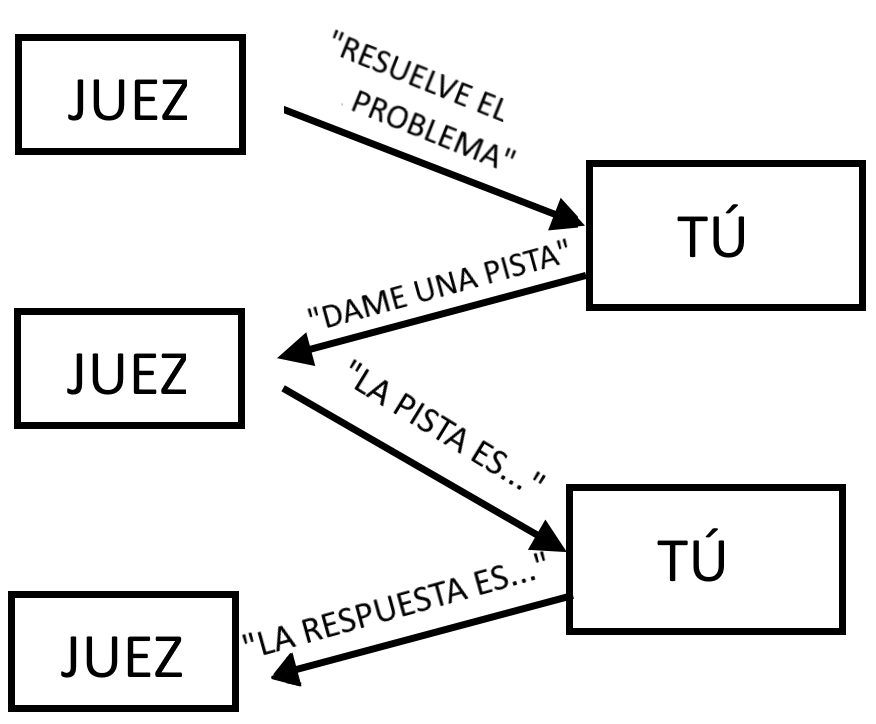
\includegraphics[scale=0.36]{interactivo1}
\end{center}

Como esto es implementado difiere un poco de juez a juez, pero en la OMI y la IOI se logra con el uso de funciones.

Tu tarea será implementar funciones que deben hacer lo que te pida el problema. Estas serán las que el juez utilizara para interactuar contigo.

Por ejemplo "resuelve el problema" podría verse como una función: int resuelve(int N) que se llamará al inicio para indicarte que resuelvas el problema, deberá retornar la solución.

Mientras que el problema te dirá que podrás llamar a funciones implementadas por el evaluador. Estas son las funciones con las cuales tú te comunicaras con el juez.

Por ejemplo: int pista(int x) es una función que te regresará algún tipo de pista que tu podrás usar para calcular la respuesta.

Veamos un ejemplo:
\subsection*{Ejemplo: Cluedo}
\addcontentsline{toc}{subsection}{Ejemplo}
El Dr. Negro ha sido asesinado. La detective Jill debe determinar el culpable, la ubicación y el arma del crimen. Existen seis posibles culpables, numerados del 1 al 6. Hay diez posibles ubicaciones, numeradas del 1 al 10. Existen 6 posibles armas homicidas, numeradas del 1 al 6. Para ilustrar, se muestran los nombres de los posibles culpables, ubicaciones y armas del crimen. Los nombres no son requeridos para resolver esta tarea.
\begin{center}
	\begin{scriptsize}
		\begin{tabular}{|l|l|l|}	
			\hline
			\thead{Culpable}&\thead{Ubicación}&\thead{Arma Homicida}\\
			\hline
			\makecell[l]{
				1. Profesor Ciruela\\
				2. Señorita Escarlata\\
				3. Coronel Mostaza\\
				4. Señora Blanca\\
				5. Reverendo verde\\
				6. Señora Pavo Real
			}&
			\makecell[l]{
				1. Salón\\
				2. Comedor\\
				3. Cocina\\
				4. Conservatorio\\
				5. Sala de Billar\\
				6. Biblioteca\\
				7. Sala de Baile \\
				8. Vestíbulo \\
				9. Estudio \\
				10. Bodega
			}&
			\makecell[l]{
				1. Daga\\
				2. Soga \\
				3. Revólver \\
				4. Candelabro\\
				5. Llave Inglesa \\
				6. Tubería
			}
			\\
			\hline
		\end{tabular}
	\end{scriptsize}
\end{center}

Jill intenta repetidas veces adivinar la combinación correcta de culpable, ubicación y arma homicida. Cada intento de adivinar es llamado una teoría. Ella le pregunta a su asistente Jack que confirme o refute la teoría que tiene. Cuando Jack confirma una teoría, Jill ha resuelto el caso. Cuando Jack refuta una teoría, le presenta a Jill evidencia de que alguno de los elementos de la teoría es incorrecto.

Tu tarea es implementar un procedimiento ResolverCaso() que juegue el papel de Jill. El evaluador llamará a tu procedimiento ResolverCaso() varias veces, cada vez con un nuevo caso por resolver. ResolverCaso() puede llamar repetidas veces a la función Teoria(c, u, a), que está implementada de manera interna en el evaluador. c, u y a son enteros denotando una combinación en particular de culpable, ubicación y arma homicida. Teoria(c, u, a) devolverá un entero, 0 si la teoría que presentes es correcta. Si la teoría es incorrecta, devolverá un valor 1, 2, o 3. El valor 1 indica que el culpable es incorrecto; 2 indica que la ubicación es incorrecta; 3 indica que el arma homicida es incorrecta. Si más de un elemento en la teoría es incorrecto, Jack elige uno al azar entre los que estén mal. Cuando una llamada a Teoria(c, u, a) devuelva 0, tu procedimiento ResolverCaso() deberá retornar.

\subsection*{Implementación}
\paragraph{Tu procedimiento:} \verb|void ResolverCaso()|
\begin{quotation}
	
\subsubsection*{Descripción}

Cada vez que Jill reciba un nuevo caso se llamará a este procedimiento, el cual deberás resolver. \textit{Asegurate de inicializar cualquier variable que uses durante cada una de las llamadas a este procedimiento.}

\subsubsection*{Parámetros}
\begin{plimits}
	\item Este procedimiento no recibe parámetros.
\end{plimits}
\end{quotation}

\paragraph{Función del evaluador:} \verb|int Teoria(int c, int u, int a)|
\begin{quotation}
\subsubsection*{Descripción}
Llama a esta función para probar una teoría sobre el homicidio. La función te devolverá un valor entero. 0 cuando la teoría es correcta (recuerda terminar la ejecución cuando resuelvas el caso); 1 si el culpable es incorrecto; 2 si la ubicación es incorrecta; 3 si el arma homicida es incorrecta.
\subsubsection*{Parámetros}
\begin{plimits}
	\item \verb|c|: La suposición del sospechoso.
	\item \verb|u|: La suposición de la ubicación.
	\item \verb|a|: La suposición del arma homicida.
\end{plimits}
\end{quotation}

\subsection*{Rutina de ejemplo}
Como ejemplo, asume que la Señorita Escarlata asesinó al Dr. Negro en la cocina usando un candelabro. Cuando el procedimiento ResolverCaso() haga las siguientes teorías, los valores devueltos serán:

\begin{tabular}{|l|l|l|}
	\hline
	\thead{Funcion} & \thead{Valor\\ retornado} & \thead{Explicación}\\
	\hline
	ResolverCaso() & - & Jill tiene un nuevo caso por resolver.\\
	\hline
	Teoria(1, 1, 1) & 1, 2 o 3 & \makecell[l]{Todo es incorrecto} \\
	\hline
	Teoria(3, 3, 3) & 1 o 3 & \makecell[l]{Solo la ubicación es correcta} \\
	\hline
	Teoria(5, 3, 4) & 1 & \makecell[l]{Solo el culpable es incorrecto} \\
	\hline
	Teoria(2, 3, 4) & 0 & \makecell[l]{Todo es correcto.} \\
	\hline	
\end{tabular}

\subsection*{Límites}
Se llamará a tu procedimiento ResolverCaso() un máximo de \(360\) veces.
\subsection*{Subtareas}
\subsubsection*{Subtarea 1 [50 puntos]}
Por cada llamada a ResolverCaso(), puedes llamar a Teoria() a lo más \(360\) veces.
\subsubsection*{Subtarea 2 [50 puntos]}
Por cada llamada a ResolverCaso(), puedes llamar a Teoria() a lo más \(20\) veces.

Fuente: IOI 2010

\omegalink{Cluedo}

\problembreak

\subsection*{Compilar y probar interactivos}
\addcontentsline{toc}{subsection}{Compilar y probar interactivos}
En omegaup, el juez utilizado para la OMI hay dos formas de programar y trabajar con problemas interactivos.

La primera forma es descargar la plantilla en la parte de abajo del problema. Elige C++ y tu sistema operativo.

Se te descargará un archivo comprimido que deberás descomprimir en alguna carpeta de tu elección.

En esta carpeta verás que dentro hay varios archivos y folders, pero a nosotros solo nos interesan unos cuantos. 

Principalmente, debemos ver un archivo \verb|.cpp|: \verb|cluedo.cpp|, este será el archivo en el cual deberás programar y enviar a omegaup. 

Si tenemos CodeBlocks instalado, recomendamos utilizar este, para esto abres el archivo \verb|.cbp|, una vez abierto esto verás a la izquierda 	los archivos de interés, Sources/problem.cpp.

Si no tenemos CodeBlocks, podemos trabajar de todas formas usando algún editor de texto y teniendo el compilador de C++ instalado, abriendo el archivo que tenga el nombre del problema + \verb|.cpp|

Para cluedo, este archivo se llamará cluedo.cpp y al abrirlo verás:

\begin{lstlisting}
	#include "cluedo.h"
	
	// Main
	//	int Teoria(int c, int u, int a)
	
	void ResolverCaso() {
		// FIXME
	}
\end{lstlisting}

La función \verb|ResolverCaso| que dice \verb|FIXME| es donde deberás escribir el código que resuelva el problema, para saber que debe hacer \verb|ResolverCaso| lee la parte de implementación del problema. 

El comentario que dice \verb|//MAIN| enlista las funciones que existen a tu disposición implementadas por el evaluador. Estas funciones las tienes disponibles gracias al \verb|#include"cluedo.h"|, es importante no borrar esa línea de código.

Ahora pasemos a resolver el problema:

La primera solución que ha de venir en mente es hacer una búsqueda completa, probando todas las combinaciones de asesino, ubicación y arma hasta que encontremos la correcta. Como hay \(6\times 10 \times 6 = 360\) combinaciones, obtendríamos 50 puntos por esta idea.

Esto en código se vería:
\pagebreak
\begin{lstlisting}
#include "cluedo.h"

void ResolverCaso() {
	for (int c=1; c<=6; c++) {
		for (int u=1; u<=10; u++) {
			for (int a=1; a<=6; a++) {
				if (Teoria(c, u, a)==0) {
					return;	
				}
			}
		}
	}
}
\end{lstlisting}

Ahora, para probar tu código, lo que haces es ejecutarlo. Si estas en CodeBlocks, basta con compilar y ejecutar tu proyecto. Si no estas usando CodeBlocks, deberás ejecutar el script \verb|compilar| y luego el script \verb|test| desde la consola.

El programa probara tu código contra un caso de prueba y te dará información sobre como se desempeño. Si quieres cambiar el caso de ejemplo que se usa, deberás cambiar el archivo \verb|examples/sample.in|.

Para entender como se prueba tu código también podrás consultar y modificar el archivo \verb|Main.cpp|, aunque no es necesario es útil para añadir información extra de debug y entender el sample.in.


La solución a este problema se deja como reto al lector.


\newpage
\section*{Colas}
\addcontentsline{toc}{section}{Colas}
\label{queue}
La cola es una estructura de datos bastante útil para muchas técnicas y problemas, en este libro se le da el principal uso para la BFS.

La idea es muy sencilla, queremos implementar algo que se comporte como la cola en la que uno se forma para comprar boletos.

En una fila pueden suceder tres cosas: alguien nuevo se forma, el de enfrente de la fila sale de la fila y el vendedor puede ver quien esta enfrente de la fila. Nosotros queremos que nuestra cola soporte esto eventos.

Entonces la cola es una estructura que puede hacer:
\begin{plimits}
	\item Agregar algo al final de la cola.
	\item Quitar al que este enfrente de la cola.
	\item Ver que está enfrente de la cola.
	\item Saber cuantas cosas hay en la cola.
\end{plimits}

Nosotros podemos o implementar nuestra propia cola, o utilizar una que ya viene incluida en C++. En este libro usaremos la que viene en C++, pero en el libro de Estructura de Datos veremos como implementarla nosotros.

\subsection*{Usar queue}
\addcontentsline{toc}{subsection}{Usar queue}

Para utilizar la cola, primero debemos incluir la librería \verb|<queue>|. Una vez hecho esto, tendremos acceso a la cola de C++.

Para crear una cola, basta con declararla bajo un nombre y especificar que tipo de datos recibirá, para esto seguimos el formato \verb|queue<tipo> nombre;|. Veamos un ejemplo de una cola de enteros.

\begin{lstlisting}
	queue<int> colaDeEnteros;
\end{lstlisting}

A esta cola le podemos hacer las cuatro operaciones fundamentales y una extra:
\begin{plimits}
	\item \verb|.push(x)| Agregar x al final.
	\item \verb|.pop()| Quitar al frente.
	\item \verb|.front()| Ver el valor de enfrente.
	\item \verb|.size()| Obtener cuantas cosas hay en la cola.
	\item \verb|.empty()| Regresa verdadero si no hay elementos en la cola.
\end{plimits}

Veamos estas operaciones en uso

\begin{lstlisting}
	#include<iostream>
	#include<queue>	
	using namespace std;		
	int main() {
		queue<int> cola;
		cout << "cola inicia vacia: " << cola.size() << "\n";
		cola.push(5);
		cola.push(3);
		cola.push(2);
		// La cola ahora tiene al {5, 3, 2} dentro
		cout << "\n";
		cout << "Tenemos "<<cola.size() << " elementos\n";
		cout << "Enfrente esta: " << cola.front()<<"\n";
		cola.pop();
		// La cola ahora tiene {3, 2}
		
		cout << "\n";
		cout << "Quedan "<<cola.size() << " elementos\n";
		cout << "Enfrente esta: "<<cola.front()<<"\n";
		cola.push(5);
		cola.push(2);
		//La cola ahora tiene {3,2,5,2}		
		cout << "\n";
		cout << "Imprimamos y vaciemos la cola:\n";
		while (cola.empty()==false) {
			cout << " "<<cola.front()<<"\n";
			cola.pop();
		}
		return 0;		
	}
\end{lstlisting}

Este programa imprime:

\begin{lstlisting}
cola inicia vacia: 0

Tenemos 3 elementos
Enfrente esta: 5

Quedan 2 elementos
Enfrente esta: 3

Imprimamos y vaciemos la cola:
 3
 2
 5
 2

\end{lstlisting}
